\documentclass{article}

\usepackage[T1]{fontenc}
\usepackage{textcomp}

\usepackage[english]{babel}
\usepackage[utf8]{inputenc}

\usepackage{lmodern}

\usepackage{hyperref}
\hypersetup{breaklinks}
\hypersetup{pdfborder=0 0 0}

\usepackage[babel=true]{microtype}


\usepackage{amsmath}
\renewcommand{\vec}[1]{\mathbf{#1}}
\newcommand{\mat}[1]{\mathbf{#1}}
\DeclareMathOperator{\Prob}{Prob}
\newcommand{\md}{\mathrm{d}}
\newcommand{\me}{\mathrm{e}}
\newcommand{\mT}{\mathrm{T}}

\usepackage{units}
\usepackage{tikz}
\usepackage{natbib}
\usepackage{hypernat}

\allowdisplaybreaks[1]

\title{FMDV notes}
\author{Jan Medlock}


\newcommand{\comment}[1]{\textbf{[#1]}}
\DeclareMathOperator{\diag}{diag}


\begin{document}

\maketitle

\section{Model}

We built a stochastic individual-based model to capture the dynamics
of FMDV in African buffalo.  The age and sex of each buffalo is
tracked along with its immune state (\autoref{fig:diagram}): either
immune due to maternal antibodies ($M$), susceptible to infection
($S$), infectious ($I$), or recovered ($R$).  There are 5 events that
can occur to each buffalo: death, birth, waning of maternal
antibodies, infection, and recovery.

\begin{figure}
  \centering
  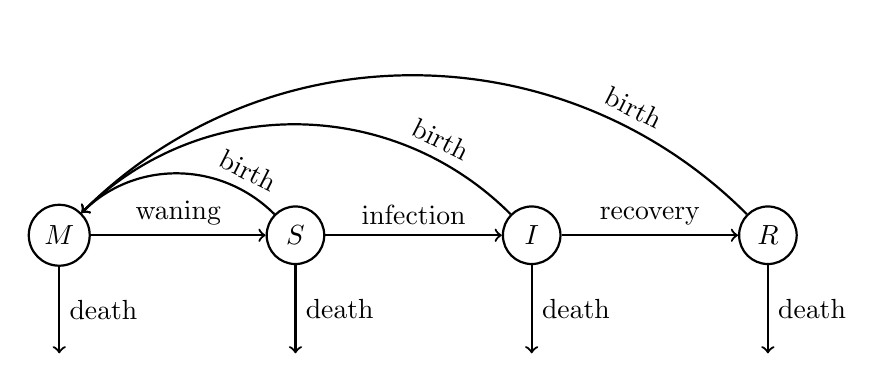
\begin{tikzpicture}[
    thick,
    compartment/.style = {circle,
      draw,
      minimum width = {width("$M$") + 10pt}}
    ]

    \node at (0, 0) [compartment, name = M] {$M$};
    \node at (3, 0) [compartment, name = S] {$S$};
    \node at (6, 0) [compartment, name = I] {$I$};
    \node at (9, 0) [compartment, name = R] {$R$};

    \draw [->] (M) to node [above] {waning} (S);
    \draw [->] (S) to node [above] {infection} (I);
    \draw [->] (I) to node [above] {recovery} (R);

    \draw [->] (S) to [out = 135, in = 45]
    node [sloped, above, pos = 0.2] {birth} (M);
    \draw [->] (I) to [out = 135, in = 45]
    node [sloped, above, pos = 0.2] {birth} (M);
    \draw [->] (R) to [out = 135, in = 45]
    node [sloped, above, pos = 0.2] {birth} (M);
    
    \draw [->] (M) to node [right] {death} +(0, -1.5);
    \draw [->] (S) to node [right] {death} +(0, -1.5);
    \draw [->] (I) to node [right] {death} +(0, -1.5);
    \draw [->] (R) to node [right] {death} +(0, -1.5);
  \end{tikzpicture}
  \caption{Model diagram.}
  \label{fig:diagram}
\end{figure}

The simulations follow a Gillespie algorithm \citep{gillespie_1977}.
\begin{description}
\item[Death] On the birth of new buffalo calf, the age at death of
  that calf is sampled from the mortality distribution.

\item[Birth] For each female buffalo, the time until she gives birth
  to a calf is sampled from its distribution.  This is done when the
  female is herself born, to find the time until she gives birth to
  her first calf, and after a birth, to find the time until she gives
  birth to her next calf.  A simple Bernoulli sample determines the
  sex of each calf.

\item[Waning] Each new buffalo calf is assumed to be immune to
  infection due to maternal antibodies: at birth, the duration of
  maternal immunity is sampled from its distribution.

\item[Infection] For each susceptible buffalo, the time to infection
  is sampled from its distribution, which depends on the current
  number of infected buffalo in the population.

\item[Recovery] On infection, the time to recovery is sampled from its
  distribution.
\end{description}
The distributions are detailed below.

For each buffalo, a list of events and the times they occur is stored.
The next event over the whole population is found and the population
is updated.  The hazards for infection depend on the number of
infectious buffalo in the population and so the times to infection are
updated after each change in the population.  The hazards of the other
events are independent of the state of the population and so the times
to these events are not updated.

This process was repeated from $t = 0$ to $t = t_{\text{max}}$ or
until there were $0$ infectious buffalo.

When sampling from simple distributions, standard algorithms were used
\citep{scipy}.  For complex distributions, the event times were
sampled using the inverse transform method \citep{rubinstein_1981}.

The variables $t$ and $a$ denote time and age, respectively, and are
both in units of years.

\subsection{Death}

We took the annual survival to be
\begin{equation}
  \Prob\{\text{Survival for $\unit[1]{yr}$}\}
  =
  \begin{cases}
    0.7 & \text{if $a < 1$},
    \\
    0.95 & \text{if $1 \leq a < 12$},
    \\
    0.5 & \text{if $a \geq 12$}.
  \end{cases}
\end{equation}
Assuming that the mortality hazard is constant throughout a year gives
the survival function for mortality
\begin{equation}
  S_{\text{mortality}}(a) =
  \begin{cases}
    0.7^a & \text{if $a < 1$},
    \\
    0.7 \cdot 0.95^a & \text{if $1 \leq a < 12$},
    \\
    0.7 \cdot 0.95^{11} \cdot 0.5^a & \text{if $a \geq 12$}.
  \end{cases}
\end{equation}
This has inverse
\begin{equation}
  Z_{\text{mortality}}(q) =
  \begin{cases}
    \unit[\frac{\log(q)}{\log(0.7)}]{yr} & \text{if $q > 0.7$},
    \\
    \unit[1 + \frac{\log(q) - \log(0.7)}{\log(0.95)}]{yr}
    & \text{if $0.7 \cdot 0.95^{11} \leq q < 0.7$},
    \\
    \unit[12 + \frac{\log(q) - \log(0.7) - 11 \log(0.95)}{\log(0.5)}]{yr}
    & \text{if $q \leq 0.7 \cdot 0.95^{11}$}.
  \end{cases}
\end{equation}


\subsection{Birth}

We assumed that females reach reproductive maturity at age $4$ and
that the birth hazard varies at a periodic, triangular-shaped rate in
time:
\begin{equation}
  h_{\text{birth}}(t, a) =
  \begin{cases}
    0 & \text{if $a < 4$},
    \\
    \mu \alpha \max\left(1 - 2 \beta \{t\}, 0\right)
    & \text{if $a \geq 4$ and $\{t\} < \frac{1}{2}$},
    \\
    \mu \alpha \max\left(1 - 2 \beta (1 - \{t\}), 0\right)
    & \text{if $\{t\} \geq \frac{1}{2}$},
  \end{cases}
\end{equation}
with
\begin{equation}
  \alpha =
  \begin{cases}
    1 + c_v \sqrt{3}
    & \text{if $c_v < \frac{1}{\sqrt{3}}$},
    \\
    \frac{3}{2} \left(1 + c_v^2\right)
    & \text{otherwise},
  \end{cases}
\end{equation}
\begin{equation}
  \beta =
  \begin{cases}
    \frac{2 c_v \sqrt{3}}{1 + c_v \sqrt{3}}
    & \text{if $c_v < \frac{1}{\sqrt{3}}$},
    \\
    \frac{3}{4} \left(1 + c_v^2\right)
    & \text{otherwise},
  \end{cases}
\end{equation}
and $\{x\}$ is the fractional part of $x$.  The magnitude of the
seasonal variation is captured by the coefficient of variation $c_v$,
which we took to be $1$ by default.  The annual mean $\mu$ was chosen
so that the population achieves the mean growth rate $r = 0$ in the
absence of infection.  (See \autoref{no_infection}.)

The survival function is then
\begin{equation}
  S_{\text{birth}}(t, a, t_0) =
  \begin{cases}
    1 & \text{if $a < 4 - t$},
    \\
    \exp(-\mu \alpha H) & \text{otherwise},
  \end{cases}
\end{equation}
where
\begin{align}
  H &=
  \begin{cases}
    H_1 + H_2  + H_3
    & \text{if $c_v < \frac{1}{\sqrt{3}}$},
    \\
    H_4 + H_5 + H_6
    & \text{otherwise},
  \end{cases}
  \\
  H_1 &= \left(1 - \frac{\beta}{2}\right)
  \left(\lfloor d \rfloor - \lfloor c \rfloor - 1\right),
  \\
  H_2 &=
  \begin{cases}
    \frac{1}{2} \left(1 - \frac{\beta}{2}\right)
    + \left(\frac{1}{2} - \{c\}\right)
    \left[1 - \beta
      + \beta \left(\frac{1}{2} - \{c\}\right)\right]
    & \text{if $\{c\} < \frac{1}{2}$},
    \\
    \left(1 - \{c\}\right)
    \left[1 - \beta + \beta \left(1 - \{c\}\right)\right]
    & \text{otherwise},
  \end{cases}
  \\
  H_3 &=
  \begin{cases}
    \{d\}\left(1 - \beta \{d\}\right)
    & \text{if $\{d\} < \frac{1}{2}$},
    \\
    \frac{1}{2} \left(1 - \frac{\beta}{2}\right)
    + \left(\{d\} - \frac{1}{2}\right)
    \left[1 - \beta
      + \beta \left(\{d\} - \frac{1}{2}\right)\right]
    & \text{otherwise},
    \end{cases}
  \\
  H_4 &= \frac{1}{2 \beta}
  \left(\lfloor d \rfloor - \lfloor c \rfloor - 1\right),
  \\
  H_5 &=
  \begin{cases}
    \frac{1}{4 \beta}
    + \beta \left(\frac{1}{2 \beta} - \{c\}\right)^2
    & \text{if $\{c\} < \frac{1}{2 \beta}$},
    \\
    \frac{1}{4 \beta}
    & \text{if $\frac{1}{2 \beta} \leq \{c\} < 1 - \frac{1}{2 \beta}$},
    \\
    \left(1 - \{c\}\right) \left[1 -
      \beta \left(1 - \{c\}\right)\right]
    & \text{otherwise}
  \end{cases},
  \\
  H_6 &=
  \begin{cases}
    \{d\} \left[1 - \beta \{d\}\right]
    & \text{if $\{d\} < \frac{1}{2 \beta}$},
    \\
    \frac{1}{4 \beta}
    & \text{if $\frac{1}{2 \beta} \leq \{d\} <
      1 - \frac{1}{2 \beta}$},
    \\
    \frac{1}{4 \beta}
    + \beta
    \left[\{d\} - \left(1 - \frac{1}{2 \beta}\right)\right]^2
    & \text{otherwise},
  \end{cases}
  \\
  c &= \max(4 - a, 0) + t_0,
  \\
  d &= t + t_0,
\end{align}
and $\lfloor x \rfloor$ is the floor function,
i.e.~$\lfloor x \rfloor = x - \{x\}$.

There is no explicit inverse survival function.  Instead, the inverse
was found numerically using a root-finding algorithm \citep{scipy}.

The probability density function is
\begin{align}
  f_{\text{birth}}(t, a, t_0) &=
  h_{\text{birth}}(t, a) S_{\text{birth}}(t, a, t_0).
\end{align}

The fraction of newborns that are male was taken to be
\begin{equation}
  p_{\text{male birth}} = 0.5.
\end{equation}


\subsection{Waning of maternal antibodies}

Immunity from maternal antibodies was assumed to last
\begin{equation}
  T_{\text{maternal immunity}} = \unit[0.5]{yr}
\end{equation}
in all buffaloes.  That is, the survival function is
\begin{equation}
  S_{\text{maternal immunity}}(t) =
  \begin{cases}
    1 & \text{if $t < 0.5$},
    \\
    0 & \text{if $t \geq 0.5$},
  \end{cases}
\end{equation}
and the inverse survival function is constant,
\begin{equation}
  Z_{\text{maternal immunity}}(q) = \unit[0.5]{yr}.
\end{equation}


\subsection{Infection}

The infection hazard was taken to be
\begin{equation}
  h_{\text{infection}}(t) = \beta I(t),
\end{equation}
where $I(t)$ is the total number of infectious buffalo in the herd at
time $t$.  Over periods where $I(t)$ is constant, the hazard is
constant, which gives an exponential random variable.

The transmission rate, $\beta$, is chosen to give the desired value of
$R_0$.  For the model,
\begin{equation}
  R_0 = \frac{\beta N}{\frac{1}{\mu_{\text{infection}}}
    + \frac{1}{\mu_{\text{mortality}}}},
\end{equation}
where $N$ is the population size,
$\mu_{\text{infection}} = \unit[1.6]{d}$ is the mean time to recovery
(see next section), and $\mu_{\text{mortality}}$ is the mean time to
death.  Thus,
\begin{equation}
  \beta = \frac{R_0}{N}
  \left(\frac{1}{\mu_{\text{infection}}} +
    \frac{1}{\mu_{\text{mortality}}}\right)
  \approx \frac{R_0}{N \mu_{\text{infection}}},
\end{equation}
because $\mu_{\text{infection}} \ll \mu_{\text{mortality}}$.

\subsection{Recovery}

The duration of infection was taken to be
\begin{equation}
  T_{\text{recovery}} = \unit[1.6]{d}
\end{equation}
in all buffaloes.  That is, the survival function is
\begin{equation}
  S_{\text{recovery}}(t) =
  \begin{cases}
    1 & \text{if $t < \frac{1.6}{365}$},
    \\
    0 & \text{if $t \geq \frac{1.6}{365}$},
  \end{cases}
\end{equation}
and the inverse survival function is constant,
\begin{equation}
  Z_{\text{recovery}}(q) = \unit[1.6]{d}.
\end{equation}


\subsection{Initial conditions}

A sample of size $N$ from the stable age structure was used to
initialize the population.  (See \autoref{no_infection}.)  The sex of
each buffalo was randomly selected with probability
$p_{\text{male birth}}$ of being male.  The simulations were started
at $t = 0$ with $2$ initial infections in randomly chosen members of
the population.

Gap sizes 7 months and greater have period-2 stable limit-cycle
asymptotic behavior.


\begin{figure}
  \centering
  \includegraphics[width = \textwidth]{hazards}
  \caption{Hazard functions.}
  \label{fig:hazard}
\end{figure}


\begin{figure}
  \centering
  \includegraphics[width = \textwidth]{survivals}
  \caption{Survival functions.}
  \label{fig:survival}
\end{figure}



\clearpage
\section{Analysis}

\subsection{No infection}
\label{no_infection}

In the absence of infection, the mean number of female births $B(t)$
follows the Lotka equation
\begin{equation}
  \label{lotka}
  \begin{split}
    B(t) =&
    \int_0^t B(t - a) S_{\text{mortality}}(a) h_{\text{birth}}(t, a) \md a
    \\
    & {} +
    \int_0^{\infty} n_0(a) \frac{S_{\text{mortality}}(a +
      t)}{S_{\text{mortality}}(a)} h_{\text{birth}}(t, a + t) \md a,
  \end{split}
\end{equation}
where $n_0(a)$ is the number of age $a$ females at time $t = 0$
\citetext{\citealp[Chapter VI, Section 29 on
  pp.~159--161]{harris_1963};
  \citealp[Chapter 20 on pp.~353--364]{kot_01}}.
% For large $t$, the contribution of the initial cohort---the second
% integral in \eqref{lotka}---becomes negligible, so
% \begin{equation}
%   B(t) =
%   \int_0^t B(t - a) \hat{h}_{\text{birth}}(t, a) \md a
% \end{equation}
% for large $t$,
% where
% \begin{equation}
%   \hat{h}_{\text{birth}}(t, a) = 
%   S_{\text{mortality}}(a) 
%   h_{\text{birth}}(t, a).
% \end{equation}
% Alternately,
% \begin{equation}
%   B(t)
%   =
%   \int_0^{t}
%   B(u)
%   \hat{h}_{\text{birth}}(t, t - u)
%   \md u.
% \end{equation}
Given $B(t)$, the mean number of females of age $a$ is
\begin{equation}
  n(t, a) =
  \begin{cases}
    B(t - a) S_{\text{mortality}}(a)
    & \text{if $a < t$},
    \\
    n_0(a - t)
    \frac{S_{\text{mortality}}(a)}{S_{\text{mortality}}(a - t)}
    & \text{if $a > t$}.
  \end{cases}
\end{equation}
The mean number of females of age $a$ satisifies the McKendrick--von
Foerster equation
\begin{equation}
  \begin{split}
    \frac{\partial n}{\partial t} + \frac{\partial n}{\partial a}
    &= - h_{\text{death}}(a) n(t, a),
    \\
    n(t, 0) &= \int_0^t n(t, a) h_{\text{birth}}(t, a) \md a,
    \\
    n(0, a) &= n_0(a).
  \end{split}
\end{equation}

Discretizing in $a$ by setting
\begin{equation}
  \label{eq:11}
  \vec{a} = \left[0, \Delta a, 2 \Delta a, \cdots, a_{\text{max}} \right]^{\mT}
\end{equation}
and
\begin{equation}
  \vec{n}(t) \approx n(t, \vec{a})
\end{equation}
gives
\begin{equation}
  \begin{split}
    \frac{\md \vec{n}}{\md t} &=
    \left[\mat{B}(t)
      - \mat{M}
      + \mat{A}\right] \vec{n},
  \end{split}
\end{equation}
with
\begin{equation}
  \begin{split}
    \mat{B}(t)
    &=
    (1 - p_{\text{male birth}})
    \begin{bmatrix}
      \cdots & h_{\text{birth}}(t, \vec{a}) & \dots
      \\
      \cdots & 0 & \cdots
      \\
      \cdots & 0 & \cdots
      \\
      & \vdots &
      \\
      \cdots & 0 & \cdots
    \end{bmatrix},
    \\
    \mat{M} &=
    \operatorname{diag}\left(h_{\text{mortality}}(\vec{a})\right),
    \\
    \mat{A} &=
    \frac{1}{\Delta a}
    \begin{bmatrix}
      -1 & 0 & 0 & 0 & \cdots & 0 & 0
      \\
      1 & -1 & 0 & 0 & \cdots & 0 & 0
      \\
      0 & 1 & -1 & 0 & \cdots & 0 & 0
      \\
      \vdots & \ddots & \ddots & \ddots & \ddots &  & \vdots
      \\
      \vdots &  & \ddots & \ddots & \ddots & \ddots & \vdots
      \\
      0  & \cdots & \cdots & 0 & 1 & - 1 & 0
      \\
      0  & \cdots & \cdots & \cdots & 0 & 1 & 0
    \end{bmatrix},
  \end{split}
\end{equation}
Solving this from $t_0$ to $t_0 + 1$ gives
\begin{equation}
  \vec{n}(t_0 + 1) = \vec{n}(t_0)
  \exp\left(\bar{\mat{B}} - \mat{M} + \mat{A}\right)
\end{equation}
where
\begin{equation}
  \begin{split}
    \bar{\mat{B}} &=
    \int_{t_0}^{t_0 + 1} \mat{B}(t) \md t =
    (1 - p_{\text{male birth}})
    \begin{bmatrix}
      \cdots & \bar{h}_{\text{birth}}(\vec{a}) & \dots
      \\
      \cdots & 0 & \cdots
      \\
      \cdots & 0 & \cdots
      \\
      & \vdots &
      \\
      \cdots & 0 & \cdots
    \end{bmatrix},
    \\
    \bar{h}_{\text{birth}}(a) &=
    \int_{t_0}^{t_0 + 1} h_{\text{birth}}(t, a + t) \md t
    \\
    &=
    \begin{cases}
      0 & \text{if $a < 3$},
      \\
      \alpha \left(
        a - 3 + \frac{\sigma}{2 \pi}
        \left[
          \sin\left(2\pi t_0\right)
          - \sin\left(2 \pi (t_0 - a)\right)
        \right]
      \right)
      & \text{if $3 \leq a < 4$},
      \\
      \alpha & \text{if $a \geq 4$}.
    \end{cases}
  \end{split}
\end{equation}
Assuming the stable age distribution so that
\begin{equation}
  \vec{n}(t_0 + 1) = \me^r \vec{n}(t_0)
\end{equation}
gives
\begin{equation}
  r = \lambda_0\left(\bar{\mat{B}} - \mat{M} + \mat{A}\right),
\end{equation}
where $\lambda_0(\mat{X})$ is the eigenvalue of $\mat{X}$ with largest
magnitude.  The eigenvector corresponding to this eigenvalue is the
stable age distribution $\vec{n}_{\text{stable}}$.

We numerically computed the eigenvalue and eigenvector by using age
steps $\Delta a = 0.01$, maximum age $a_{\text{max}} = 20$
(probability of survival $S_{\text{mortality}}(20) = 0.0016$), and a
standard eigenvalue solver
\citep[\texttt{numpy.linalg.eig},][]{scipy}.  We then used a standard
root-finding algorithm
\citep[\texttt{scipy.optimize.fsolve},][]{scipy} to find the value of
the mean birth hazard $\mu \approx 0.443$ that gave growth rate
$r = 0$.  Halving the age step to $\Delta a = 0.005$ gave a value of
$\mu$ within $1.2 \times 10^{-4}$ and doubling the maximum age to
$a_{\text{max}} = 40$ gave a value of $\mu$ within
$1.7 \times 10^{-12}$.


\subsection{$R_0$}


\appendix

\section{Alternate Birth Hazards}

\subsection{Rectangular}

Let the hazard be constant $\alpha$ in the regions of width
$\beta \in (0, 1]$ centered at $\{t\} = 0$ and $0$ elsewhere:
\begin{equation}
  h_{\text{birth}} (t, a) =
  \begin{cases}
    \alpha & \text{if $a \geq 4$ and $\left\{t + \frac{\beta}{2}\right\}
      \leq \beta$},
    \\
    0 & \text{otherwise},
  \end{cases}
\end{equation}
where $\{x\}$ is the fractional part of $x$.  For $a > 4$, the mean
and variance are
\begin{align}
  \mu &= \alpha \beta,
  &
  \sigma^2 &= \alpha^2 \beta (1 - \beta),
\end{align}
so the coefficient of variation is
\begin{equation}
  c_v = \sqrt{\frac{1 - \beta}{\beta}},
\end{equation}
which gives
\begin{align}
  \alpha &= \mu \left(1 + c_v^2\right),
  &
  \beta &= \frac{1}{1 + c_v^2}.
\end{align}
With $\mu$ fixed, this gives one parameter, $c_v$.

The survival is
\begin{equation}
  S_{\text{birth}}(t, a, t_0) =
  \begin{cases}
    1 & \text{if $a < 4 - t$},
    \\
    \exp\left(-H(t, a, t_0)\right)
    & \text{otherwise},
  \end{cases}
\end{equation}
where
\begin{equation}
  H(t, a, t_0) =
  \alpha \left[
    \beta (\lfloor d \rfloor - \lfloor c \rfloor)
    + \min(\{d\}, \beta)
    - \min(\{c\}, \beta)
  \right]
\end{equation}
and
\begin{align}
  c &= \max(4 - a, 0) + t_0 + \frac{\beta}{2},
  &
  d &= t + t_0 + \frac{\beta}{2}.
\end{align}



\subsection{Triangular}

Let the hazard be triangular with maximum $\alpha$ and slopes
$\pm 2 \alpha \beta$ centered at $t = 0$:
\begin{equation}
  h_{\text{birth}} (t, a) =
  \begin{cases}
    0 & \text{if $a < 4$},
    \\
    \alpha \max\left(1 - 2 \beta \{t\}, 0\right)
    & \text{if $a \geq 4$ and $\{t\} < \frac{1}{2}$},
    \\
    \alpha \max\left(1 - 2 \beta (1 - \{t\}), 0\right)
    & \text{if $a \geq 4$ and $\{t\} \geq \frac{1}{2}$}.
  \end{cases}
\end{equation}

\subsubsection{$\beta \leq 1$}

With $\beta \leq 1$, the $\max(x, 0) = x$ in the hazard:
\begin{equation}
  h_{\text{birth}} (t, a) =
  \begin{cases}
    0 & \text{if $a < 4$},
    \\
    \alpha \left(1 - 2 \beta \{t\}\right)
    & \text{if $a \geq 4$ and $\{t\} < \frac{1}{2}$},
    \\
    \alpha \left[1 - 2 \beta (1 - \{t\})\right]
    & \text{if $a \geq 4$ and $\{t\} \geq \frac{1}{2}$}.
  \end{cases}
\end{equation}
For $a > 4$, the mean is
\begin{align}
  \mu = \int_0^1 h_{\text{birth}}(t, a) \; \md t
  = 2 \alpha \int_0^{\frac{1}{2}} 1 - 2 \beta t \; \md t
  % = 2 a \left[t - b t^2\right]_0^{\frac{1}{2}}
  = \frac{\alpha (2 - \beta)}{2}
\end{align}
and
\begin{align}
  \int_0^1 \left[h_{\text{birth}}(t, a)\right]^2 \md t
  % \\
  = 2 \alpha^2 \int_0^{\frac{1}{2}} \left(1 - 2 \beta t\right)^2 \md t
  % \\
  % &= 2 a^2 \int_0^{\frac{1}{2}} 1 - 4 b t + 4 b^2 t^2 \; \md t
  % \\
  % &= 2 a^2 \left[t - 2 b t^2 + \frac{4 b^2}{3} t^3\right]_0^{\frac{1}{2}}
  % \\
  = \frac{\alpha^2 (\beta^2 - 3 \beta + 3)}{3}
\end{align}
so the variance is
\begin{align}
  \sigma^2
  % &= \frac{a^2}{3} (b^2 - 3 b + 3) - \frac{a^2}{4} (2 - b)^2
  % \\
  &= \frac{\alpha^2 \beta^2}{12}
\end{align}
and the coefficient of variation is
\begin{equation}
  c_v = \frac{\beta}{(2 - \beta) \sqrt{3}}.
\end{equation}
Then
\begin{align}
  \alpha &= \mu \left(1 + c_v \sqrt{3}\right),
  &
  \beta &= \frac{2 c_v \sqrt{3}}{1 + c_v \sqrt{3}}.
\end{align}

The survival is
\begin{equation}
  S_{\text{birth}}(t, a, t_0) =
  \begin{cases}
    1 & \text{if $a < 4 - t$},
    \\
    \exp(-\alpha H) & \text{otherwise},
  \end{cases}
\end{equation}
where
\begin{equation}
  H =
  \int_{\ell}^t g(t_0 + \tau)~\md \tau,
\end{equation}
\begin{equation}
  g (t) =
  \begin{cases}
    1 - 2 \beta \{t\}
    & \text{if $\{t\} < \frac{1}{2}$},
    \\
    1 - 2 \beta (1 - \{t\})
    & \text{if $\{t\} \geq \frac{1}{2}$},
  \end{cases}
\end{equation}
and
\begin{equation}
  \ell = \max(4 - a, 0).
\end{equation}
Then
\begin{equation}
  H = H_1  + H_2 + H_3,
\end{equation}
with
\begin{align}
  H_1 &= \left(1 - \frac{\beta}{2}\right)
  \left(\lfloor d \rfloor - \lfloor c \rfloor - 1\right),
  \\
  H_2 &=
  \begin{cases}
    \frac{1}{2} \left(1 - \frac{\beta}{2}\right)
    + \left(\frac{1}{2} - \{c\}\right)
    \left[1 - \beta
      + \beta \left(\frac{1}{2} - \{c\}\right)\right]
    & \text{if $\{c\} < \frac{1}{2}$},
    \\
    \left(1 - \{c\}\right)
    \left[1 - \beta + \beta \left(1 - \{c\}\right)\right]
    & \text{otherwise},
  \end{cases}
  \\
  H_3 &=
  \begin{cases}
    \{d\}\left(1 - \beta \{d\}\right)
    & \text{if $\{d\} < \frac{1}{2}$},
    \\
    \frac{1}{2} \left(1 - \frac{\beta}{2}\right)
    + \left(\{d\} - \frac{1}{2}\right)
    \left[1 - \beta
      + \beta \left(\{d\} - \frac{1}{2}\right)\right]
    & \text{otherwise},
    \end{cases}
\end{align}
and
\begin{align}
  c &= \ell + t_0 = \max(4 - a, 0) + t_0,
  &
  d &= t + t_0.
\end{align}


\subsubsection{$\beta \geq 1$}

Here we have
\begin{equation}
  h_{\text{birth}}(t, a) =
  \begin{cases}
    0 & \text{if $a < 4$},
    \\
    \alpha \left(1 - 2 \beta \{t\}\right)
    & \text{if $a \geq 4$ and $\{t\} < \frac{1}{2 \beta}$},
    \\
    \alpha \left[1 - 2 \beta (1 - \{t\})\right]
    & \text{if $\{t\} \geq 1 - \frac{1}{2 \beta}$},
    \\
    0 & \text{otherwise}.
  \end{cases}
\end{equation}
For $a \geq 4$, the mean is
\begin{align}
  \mu = \int_0^1 h_{\text{birth}}(t, a) \md t
  = 2 \alpha \int_0^{\frac{1}{2 \beta}} 1 - 2 \beta t \; \md t
  = \frac{\alpha}{2 \beta}
\end{align}
and
\begin{align}
  \int_0^1 \left[h_{\text{birth}}(t, a)\right]^2 \md t
  & = 2 \alpha^2 \int_0^{\frac{1}{2 \beta}} \left(1 - 2 \beta t\right)^2 \md t
  % \\
  % &= 2 a^2 \int_0^{\frac{1}{2 c}} 1 - 4 c t + 4 c^2 t^2
  %   \; \md t
  % \\
  % &= 2 a^2 \left[t - 2 c t^2 + \frac{4 c^2}{3} t^3\right]_0^{\frac{1}{2 c}}
  % \\
  = \frac{\alpha^2}{3 \beta},
\end{align}
so the variance is
\begin{align}
  \sigma^2 = \frac{\alpha^2}{12 \beta^2} (4 \beta - 3)
\end{align}
and the coefficient of variation is
\begin{equation}
  c_v = \sqrt{\frac{4 \beta - 3}{3}}.
\end{equation}
This gives
\begin{align}
  \alpha &= \frac{3}{2} \mu \left(1 + c_v^2\right),
  &
  \beta &= \frac{3}{4} \left(1 + c_v^2\right).
\end{align}

The survival is
\begin{equation}
  S_{\text{birth}}(t, a, t_0) =
  \begin{cases}
    1 & \text{if $a < 4 - t$},
    \\
    \exp(-\alpha H) & \text{otherwise},
  \end{cases}
\end{equation}
where
\begin{equation}
  H = \int_{\ell}^t g(t_0 + \tau)~\md \tau,
\end{equation}
\begin{equation}
  g (t) =
  \begin{cases}
    1 - 2 \beta \{t\}
    & \text{if $\{t\} < \frac{1}{2 \beta}$},
    \\
    1 - 2 \beta (1 - \{t\})
    & \text{if $\{t\} \geq 1 - \frac{1}{2 \beta}$},
    \\
    0 & \text{otherwise},
  \end{cases}
\end{equation}
and
\begin{equation}
  \ell = \max(4 - a, 0).
\end{equation}
Then
\begin{equation}
  H = H_4 + H_5 + H_6,
\end{equation}
with
\begin{align}
  H_4 &= \frac{1}{2 \beta}
  \left(\lfloor d \rfloor - \lfloor c \rfloor - 1\right),
  \\
  H_5 &=
  \begin{cases}
    \frac{1}{4 \beta}
    + \beta \left(\frac{1}{2 \beta} - \{c\}\right)^2
    & \text{if $\{c\} < \frac{1}{2 \beta}$},
    \\
    \frac{1}{4 \beta}
    & \text{if $\frac{1}{2 \beta} \leq \{c\} < 1 - \frac{1}{2 \beta}$},
    \\
    \left(1 - \{c\}\right) \left[1 -
      \beta \left(1 - \{c\}\right)\right]
    & \text{otherwise}
  \end{cases},
  \\
  H_6 &=
  \begin{cases}
    \{d\} \left[1 - \beta \{d\}\right]
    & \text{if $\{d\} < \frac{1}{2 \beta}$},
    \\
    \frac{1}{4 \beta}
    & \text{if $\frac{1}{2 \beta} \leq \{d\} <
      1 - \frac{1}{2 \beta}$},
    \\
    \frac{1}{4 \beta}
    + \beta
    \left[\{d\} - \left(1 - \frac{1}{2 \beta}\right)\right]^2
    & \text{otherwise},
  \end{cases}
  \\
  c &= \max(4 - a, 0) + t_0,
  \\
  d &= t + t_0,
\end{align}
and
\begin{align}
  c &= \ell + t_0 = \max(4 - a, 0) + t_0,
  &
  d &= t + t_0.
\end{align}


\subsection{Sinusoidal}

We assumed that females reach reproductive maturity at age $4$ and
that the birth hazard varies sinusoidally in time:
\begin{equation}
  h_{\text{birth}}(t, a) =
  \begin{cases}
    0 & \text{if $a < 4$},
    \\
    \alpha \left[1
      + 2 c_v \cos\left(2 \pi t\right)\right]
    & \text{if $a \geq 4$}.
  \end{cases}
\end{equation}
The seasonal variation is captured by the coefficient of variation
$c_v \in \left[0, \frac{1}{2}\right]$, which we took to be
$\frac{1}{2}$ by default.  The annual mean $\alpha$ was chosen so that
the population achieves the mean growth rate $r = 0$ in the absence of
infection.  (See \autoref{no_infection}.)

The survival function is then
\begin{equation}
  \begin{split}
    S_{\text{birth}}(t, a, t_0) &=
    \exp\left(- \int_0^t h_{\text{birth}}(t_0 + \tau, a + \tau) \md
      \tau\right)
    \\
    &=
    \begin{cases}
      1 & \text{if $a < 4 - t$},
      \\
      \exp\left(- \alpha \left[
          (t - \ell)
          + \frac{c_V}{\pi}
          \left[\sin\left(2 \pi (t + t_0)\right)
            - \sin\left(2 \pi (t_0 + \ell)\right)\right]
        \right]
      \right)
      & \text{if $a \geq 4 - t$},
    \end{cases}
  \end{split}
\end{equation}
with $\ell = \max\{0, 4 - a\}$.  There is no explicit inverse survival
function.  Instead, the inverse was found numerically using a
root-finding algorithm \citep{scipy}.



\section{Finite-difference method}

\subsection{Explicit}

For the McKendrick--von Foerster equation
\begin{equation}
  \begin{split}
    \frac{\partial u}{\partial t} + \frac{\partial u}{\partial a}
    &= f(a, u),
    \\
    u(t, 0) &= \int_0^t B(t, a) u(t, a) \md a,
    \\
    u(0, a) &= u_0(a),
  \end{split}
\end{equation}
for the approximation
\begin{equation}
  u(n \Delta t, i \Delta a) \approx U_i^n,
\end{equation}
we will use a forward difference in time,
\begin{equation}
  \frac{\partial u}{\partial t} (n \Delta t, i \Delta a)
  \approx
  \frac{U^{n + 1}_i - U^n_i}{\Delta t},
\end{equation}
and a backward difference in age,
\begin{equation}
  \frac{\partial u}{\partial a} (n \Delta t, i \Delta a)
  \approx
  \frac{U^n_i - U^n_{i - 1}}{\Delta a}.
\end{equation}
Letting
\begin{equation}
  f\left(i \Delta a, u(n \Delta t, a)\right)
  \approx F_i(\vec{U}^n)
\end{equation}
gives
\begin{equation}
  \frac{U^{n + 1}_i - U^n_i}{\Delta t}
  +
  \frac{U^n_i - U^n_{i - 1}}{\Delta a}
  = F_i(\vec{U}^n).
\end{equation}
Alternately
\begin{equation}
  U^{n + 1}_i
  =
  \left(1 - \frac{\Delta t}{\Delta a}\right)
  U^n_i
  +
  \frac{\Delta t}{\Delta a} U^n_{i - 1} + \Delta t \, F_i(\vec{U}^n),
\end{equation}
or
\begin{equation}
  \vec{U}^{n + 1}
  =
  \mat{A} \vec{U}^{n} + \Delta t \, \vec{F}(\vec{U}^n),
\end{equation}
with
\begin{equation}
  \mat{A} =
  \begin{bmatrix}
    1 - \frac{\Delta t}{\Delta a} & 0
    & \hdotsfor{3} & 0
    \\
    \frac{\Delta t}{\Delta a} & 1 - \frac{\Delta t}{\Delta a} & 0
    & \hdotsfor{2} & 0
    \\
    0 & \frac{\Delta t}{\Delta a} & 1 - \frac{\Delta t}{\Delta a} & 0
    & \hdots & 0
    \\
    \vdots & \ddots & \ddots & \ddots & \ddots & \vdots
    \\
    0 & \hdots & 0 & \frac{\Delta t}{\Delta a}  & 1 - \frac{\Delta
      t}{\Delta a} & 0
    \\
    0 & \hdotsfor{2} & 0 & \frac{\Delta t}{\Delta a} & 1
  \end{bmatrix}.
\end{equation}


\subsection{Implicit}

For the McKendrick--von Foerster equation
\begin{equation}
  \begin{split}
    \frac{\partial u}{\partial t} + \frac{\partial u}{\partial a}
    &= f(a, u),
    \\
    u(t, 0) &= \int_0^t B(t, a) u(t, a) \md a,
    \\
    u(0, a) &= u_0(a),
  \end{split}
\end{equation}
for the approximation
\begin{equation}
  u(n \Delta t, i \Delta a) \approx U_i^n,
\end{equation}
we will use a backward difference in time,
\begin{equation}
  \frac{\partial u}{\partial t} (n \Delta t, i \Delta a)
  \approx
  \frac{U^n_i - U^{n - 1}_i}{\Delta t},
\end{equation}
and a forward difference in age,
\begin{equation}
  \frac{\partial u}{\partial a} (n \Delta t, i \Delta a)
  \approx
  \frac{U^n_{i + 1} - U^n_i}{\Delta a}.
\end{equation}
Letting
\begin{equation}
  f\left(i \Delta a, u(n \Delta t, a)\right)
  \approx F_i(\vec{U}^{n - 1}, \vec{U}^n)
\end{equation}
gives
\begin{equation}
  \frac{U^n_i - U^{n - 1}_i}{\Delta t}
  +
  \frac{U^n_{i + 1} - U^n_i}{\Delta a}
  = F_i(\vec{U}^{n - 1}, \vec{U}^n).
\end{equation}
Alternately
\begin{equation}
  \frac{\Delta t}{\Delta a} U^n_{i + 1}
  +
  \left(1 - \frac{\Delta t}{\Delta a}\right)
  U^n_i
  =
  U^{n - 1}_i + \Delta t \, F_i(\vec{U}^{n - 1}, \vec{U}^n),
\end{equation}
or
\begin{equation}
  \mat{A} \vec{U}^n
  =
  \vec{U}^{n - 1} + \Delta t \, \vec{F}(\vec{U}^{n - 1}, \vec{U}^n),
\end{equation}
with
\begin{equation}
  \mat{A} =
  \begin{bmatrix}
    1 - \frac{\Delta t}{\Delta a} & \frac{\Delta t}{\Delta a} & 0
    & \hdotsfor{2} & 0
    \\
    0 & 1 - \frac{\Delta t}{\Delta a} & \frac{\Delta t}{\Delta a}
    & 0 & \hdots & 0
    \\
    \vdots & \ddots & \ddots & \ddots & \ddots & \vdots
    \\
    0 & \hdots & 0 & 1 - \frac{\Delta t}{\Delta a} &
    \frac{\Delta t}{\Delta a} & 0
    \\
    0 & \hdotsfor{2} & 0 & 1 - \frac{\Delta t}{\Delta a} & \frac{\Delta t}{\Delta a}
    \\
    0 & \hdotsfor{3} & 0 & 1
  \end{bmatrix}.
\end{equation}

More concretely,
\begin{equation}
  \begin{split}
    \mat{A} \vec{S}^n
    &=
    \vec{S}^{n - 1}
    + \Delta t \, 
    \mat{F}_S(\vec{S}^{n - 1}, \vec{I}^{n - 1}, \vec{R}^{n - 1},
    \vec{S}^n, \vec{I}^n, \vec{R}^n),
    \\
    \mat{A} \vec{I}^n
    &=
    \vec{I}^{n - 1}
    + \Delta t \,
    \mat{F}_I(\vec{S}^{n - 1}, \vec{I}^{n - 1}, \vec{R}^{n - 1},
    \vec{S}^n, \vec{I}^n, \vec{R}^n),
    \\
    \mat{A} \vec{R}^n
    &=
    \vec{R}^{n - 1}
    + \Delta t \mat{F}_R(\vec{S}^{n - 1}, \vec{I}^{n - 1}, \vec{R}^{n - 1},
    \vec{S}^n, \vec{I}^n, \vec{R}^n),
  \end{split}
\end{equation}
with
\begin{equation}
  \begin{split}
    \vec{F}_S(\vec{S}^{n - 1}, \vec{I}^{n - 1}, \vec{R}^{n - 1},
    \vec{S}^n, \vec{I}^n, \vec{R}^n)
    &= \mat{B}^n (\vec{S}^n + \vec{I}^n + \vec{R}^n)
    - \mat{M} \vec{S}^n
    - {\vec{I}^{\ell}}^{\mT} \vec{T} \mat{\Sigma} \vec{S}^m
    \\
    \vec{F}_I(\vec{S}^{n - 1}, \vec{I}^{n - 1}, \vec{R}^{n - 1},
    \vec{S}^n, \vec{I}^n, \vec{R}^n)
    &= - \mat{M} \vec{I}^n
    + {\vec{I}^{\ell}}^{\mT} \vec{T} \mat{\Sigma} \vec{S}^m
    - \frac{1}{T_{\text{recovery}}} \vec{I}^n
    \\
    \vec{F}_R(\vec{S}^{n - 1}, \vec{I}^{n - 1}, \vec{R}^{n - 1},
    \vec{S}^n, \vec{I}^n, \vec{R}^n)
    &= - \mat{M} \vec{R}^n + \frac{1}{T_{\text{recovery}}} \vec{I}^n,
    \\
    \mat{M} &= \diag\left(\left\{h_{\text{mortatlity}}(i \Delta
        a)\right\}_{i = 0}^{N_a}\right),
    \\
    \mat{B}^n &=
    \begin{bmatrix}
      b^n_0
      &
      b^n_1
      &
      \hdots
      &
      b^n_{N_a}
      \\
      0 & 0 & \hdots & 0
      \\
      \vdots & \vdots & & \vdots
      \\
      0 & 0 & \hdots & 0
    \end{bmatrix},
    \\
    b^n_i &= h_{\text{birth}}(n \Delta t, i \Delta a),
    \\
    \vec{T} &= \beta \Delta a
    \begin{pmatrix}
      \frac{1}{2} \\ 1 \\ 1 \\ \vdots \\ 1 \\ \frac{1}{2}
    \end{pmatrix},
    \\
    \mat{\Sigma} &= \diag\left(
      \left\{
        \begin{array}{ll}
          0 & \text{if $i \Delta a \leq T_{\text{maternal immunity}}$}
          \\
          1 & \text{otherwise}
        \end{array}
      \right\}_{i = 0}^{N_a}
    \right),
  \end{split}
\end{equation}
and $\ell, m \in \{n - 1, n\}$.  Combining these gives
\begin{equation}
  \begin{split}
    \vec{U}^n &=
    \begin{pmatrix}
      \vec{S}^n
      \\
      \vec{I}^n
      \\
      \vec{R}^n
    \end{pmatrix},
    \\
    \mat{A}_U \vec{U}^n
    &=
    \vec{U}^{n - 1}
    + \Delta t \, \vec{F}_U(\vec{U}^{n - 1}, \vec{U}^n),
    \\
    \mat{A}_U &=
    \begin{bmatrix}
      \mat{A} & \mat{0} & \mat{0}
      \\
      \mat{0} & \mat{A} & \mat{0}
      \\
      \mat{0} & \mat{0} & \mat{A}
    \end{bmatrix},
    \\
    \vec{F}_U(\vec{U}^{n - 1}, \vec{U}^n) &=
    - \mat{M}_U \vec{U}^n  + \mat{\Gamma}_U \vec{U}^n
    + \mat{B}_U^n \vec{U}^n
    + {\vec{U}^{\ell}}^{\mT} \vec{T}_U \mat{\Sigma}_U \vec{U}^m,
    \\
    \mat{B}_U^n &=
    \begin{bmatrix}
      \mat{B}^n & \mat{B}^n & \mat{B}^n
      \\
      \mat{0} & \mat{0} & \mat{0}
      \\
      \mat{0} & \mat{0} & \mat{0}
    \end{bmatrix},
    \\
    \mat{M}_U &=
    \begin{bmatrix}
      \mat{M} & \mat{0} & \mat{0}
      \\
      \mat{0} & \mat{M} & \mat{0}
      \\
      \mat{0} & \mat{0} & \mat{M}
    \end{bmatrix},
    \\
    \mat{\Sigma}_U &=
    \begin{bmatrix}
      - \mat{\Sigma} & \mat{0} & \mat{0}
      \\
      \mat{\Sigma} & \mat{0} & \mat{0}
      \\
      \mat{0} & \mat{0} & \mat{0}
    \end{bmatrix},
    \\
    \mat{T}_U &=
    \begin{pmatrix}
      \vec{0} \\ \vec{T} \\ \vec{0}
    \end{pmatrix},
    \\
    \mat{\Gamma}_U &=
    \begin{bmatrix}
      \mat{0} & \mat{0} & \mat{0}
      \\
      \mat{0} & - \mat{\Gamma} & \mat{0}
      \\
      \mat{0} & \mat{\Gamma} & \mat{0}
    \end{bmatrix},
    \\
    \mat{\Gamma} &= \diag\left(\frac{1}{T_{\text{recovery}}}\right).
  \end{split}
\end{equation}
Thus
\begin{equation}
  \left[\mat{A}_U + \Delta t \left(\mat{M}_U - \mat{\Gamma}_U
    - \mat{B}_U^n\right)\right] \vec{U}^n
  =
  \vec{U}^{n - 1}
  + \Delta t \, {\vec{U}^{\ell}}^{\mT} \vec{T}_U \mat{\Sigma}_U \vec{U}^m.
\end{equation}

\begin{enumerate}
\item $\ell = n - 1$ and $m = n$,
  \begin{equation}
    \left[\mat{A}_U + \Delta t \left(\mat{M}_U - \mat{\Gamma}_U
        - \mat{B}_U^n
        - {\vec{U}^{n-1}}^{\mT} \vec{T}_U \mat{\Sigma}_U\right)\right] \vec{U}^n
    =
    \vec{U}^{n - 1}.
  \end{equation}
\item $\ell = m = n - 1$,
  \begin{equation}
    \left[\mat{A}_U + \Delta t \left(\mat{M}_U - \mat{\Gamma}_U
      - \mat{B}_U^n\right)\right] \vec{U}^n
    =
    \left(\mat{I}
      + \Delta t \, {\vec{U}^{n - 1}}^{\mT} \vec{T}_U \mat{\Sigma}_U\right)
    \vec{U}^{n - 1}.
  \end{equation}
% \item $\ell = n$ and $m = n - 1$,
%   \begin{equation}
%     \left[\mat{A}_U + \Delta t \left(\mat{M}_U - \mat{\Gamma}_U
%       - \mat{B}_U^n \right)\right] \vec{U}^n
%   - \Delta t \, {\vec{U}^n}^{\mT} \vec{T}_U \mat{\Sigma}_U \vec{U}^{n - 1}
%     =
%     \vec{U}^{n - 1}.
%   \end{equation}
%   I'm not sure how to handle this one.
\end{enumerate}



\bibliography{journal_abbreviations,math_epi}
\bibliographystyle{jpmbib}


\end{document}
